\documentclass{report}
\usepackage{pdfpages}
\usepackage{amssymb}
\usepackage{graphicx} 
\usepackage{dirtytalk}
\usepackage{lmodern}
\usepackage{booktabs}
\usepackage{listings}
\usepackage{float}
\usepackage{siunitx}
\usepackage{amsmath}
\usepackage{rotating}
\usepackage{arydshln}

\usepackage{listings}
\usepackage{xcolor}

\lstset{
    basicstyle=\ttfamily\small,
    breaklines=true,
    frame=single,
    language=Python,
    showstringspaces=false
}
\usepackage[hidelinks]{hyperref}
\usepackage[ngerman]{babel}
\usepackage[a4paper, total={6in, 8in}]{geometry}
\begin{document}
\begin{titlepage}
    \begin{center}
        \vspace*{1cm}
            
        \Huge
        \textbf{Versuch zu Viskosität und Reynoldszahl}
            
        \vspace{0.5cm}
        \LARGE
        Vorbereitung, Protokoll und Auswertung
        
        \vspace{1.8cm}

        \textbf{Alejandro Schultheiss}
        \vfill
            
        P1 Praktikum\\
       
            
        \vspace{0.8cm}
  

        \vspace{1.8cm}
        \Large
        LMU München \\
        Physik B.Sc.\\
        Deutschland\\
        2026
            
    \end{center}
\end{titlepage}
\tableofcontents

\newpage
\chapter{Vorbereitung und Grundlagen}

\section{Theoretische Grundlagen}

Die Viskosität beschreibt die innere Reibung einer Flüssigkeit und ist damit ein Maß für deren
Zähigkeit. Ursache dieser inneren Reibung sind die Wechselwirkungen zwischen benachbarten
Molekülen der Flüssigkeit. Bewegen sich verschiedene Flüssigkeitsschichten relativ zueinander,
so treten Reibungskräfte auf, die der Relativbewegung entgegenwirken.

\noindent
Zur quantitativen Beschreibung betrachtet man benachbarte Flüssigkeitsschichten mit dem
Geschwindigkeitsunterschied $\Delta v$ und dem Abstand $\Delta x$. Für eine Newtonsche
Flüssigkeit gilt das Newtonsche Reibungsgesetz
\begin{equation}
    F = \eta \, A \, \frac{\Delta v}{\Delta x},
\end{equation}
wobei $F$ die Reibungskraft, $A$ die Fläche der Schichten und $\eta$ die dynamische
Viskosität ist. Die Einheit der dynamischen Viskosität ist
\begin{equation}
    [\eta] = \mathrm{Pa\,s}.
\end{equation}

\noindent
Ist die Viskosität unabhängig von der Fließgeschwindigkeit, so spricht man von einer
Newtonschen Flüssigkeit. Für den vorliegenden Versuch wird diese Näherung verwendet.
Außerdem nimmt die Viskosität von Flüssigkeiten im Allgemeinen mit steigender Temperatur ab.
Daher ist zu erwarten, dass kaltes Spülmittel eine größere Viskosität besitzt als warmes.

\subsection{Laminare und turbulente Strömung}

Für die Gültigkeit der im Versuch verwendeten Modelle ist entscheidend, dass die Strömung
laminar ist. Bei laminarer Strömung gleiten die Flüssigkeitsschichten geordnet aneinander
vorbei, ohne sich makroskopisch zu verwirbeln. Bei turbulenter Strömung treten dagegen
Wirbel auf, sodass die einfachen Zusammenhänge nicht mehr unmittelbar anwendbar sind.

\noindent
Zur Charakterisierung der Strömung dient die Reynoldszahl
\begin{equation}
    \mathrm{Re} = \frac{v \, 2r \, \rho}{\eta},
\end{equation}
wobei $v$ die Geschwindigkeit des Körpers relativ zur Flüssigkeit, $r$ sein Radius,
$\rho$ die Dichte der Flüssigkeit und $\eta$ deren dynamische Viskosität ist.
Für kleine Reynoldszahlen liegt laminare Strömung vor; ab etwa
\begin{equation}
    \mathrm{Re} \gtrsim 2000
\end{equation}
ist mit turbulenter Strömung zu rechnen.

\subsection{Stokessches Gesetz}

Bewegt sich eine kleine Kugel mit geringer Geschwindigkeit durch eine ausgedehnte Flüssigkeit
und liegt laminare Strömung vor, so gilt für die viskose Reibungskraft das Stokessche Gesetz:
\begin{equation}
    F_\mathrm{R} = - 6 \pi r \eta v.
\end{equation}
Das Minuszeichen verdeutlicht, dass die Reibungskraft stets entgegengesetzt zur
Bewegungsrichtung wirkt.

\subsection{Kräftegleichgewicht beim Kugelfallviskosimeter}

Beim Kugelfallviskosimeter sinkt eine Kugel der Dichte $\rho_\mathrm{K}$ und des Radius $r$
durch die Flüssigkeit. Auf die Kugel wirken die Gewichtskraft
\begin{equation}
    F_\mathrm{G} = \frac{4}{3}\pi r^3 \rho_\mathrm{K} g,
\end{equation}
die Auftriebskraft
\begin{equation}
    F_\mathrm{A} = \frac{4}{3}\pi r^3 \rho_\mathrm{Fl} g
\end{equation}
sowie die viskose Reibungskraft nach Stokes.

\noindent
Nach einer kurzen Beschleunigungsphase stellt sich eine konstante Endgeschwindigkeit $v$ ein.
Dann ist die resultierende Kraft gleich null:
\begin{equation}
    F_\mathrm{G} - F_\mathrm{A} - F_\mathrm{R} = 0.
\end{equation}
Einsetzen der obigen Ausdrücke liefert
\begin{equation}
    \frac{4}{3}\pi r^3 (\rho_\mathrm{K} - \rho_\mathrm{Fl}) g
    = 6 \pi r \eta v.
\end{equation}
Daraus ergibt sich für die Viskosität der Flüssigkeit
\begin{equation}
    \eta = \frac{2}{9} \frac{r^2 g (\rho_\mathrm{K} - \rho_\mathrm{Fl})}{v}.
\end{equation}

\noindent
Die Geschwindigkeit wird im Experiment aus Fallstrecke $s$ und Fallzeit $t$ bestimmt:
\begin{equation}
    v = \frac{s}{t}.
\end{equation}

\subsection{Bestimmung der Viskosität über den Aufstieg von Luftblasen}

Im ersten Teilversuch wird die Viskosität des Spülmittels über den Aufstieg von Luftblasen
bestimmt. Auf eine Luftblase wirken im Wesentlichen die Auftriebskraft und die viskose
Reibungskraft. Da die Dichte der Luft gegenüber der Dichte des Spülmittels sehr klein ist,
wird die Gewichtskraft der Luftblase vernachlässigt.

\noindent
Die Auftriebskraft einer Luftblase mit Radius $r_\mathrm{B}$ in einer Flüssigkeit der Dichte
$\rho_\mathrm{Spueli}$ beträgt

\begin{equation}
    F_\mathrm{A} = \frac{4}{3}\pi r_\mathrm{B}^3 \rho_\mathrm{Spueli} g.
\end{equation}

\noindent
Bei konstanter Aufstiegsgeschwindigkeit $v_\mathrm{B}$ gilt betragsmäßig
\begin{equation}
    F_\mathrm{A} = F_\mathrm{R}.
\end{equation}
Mit dem Stokesschen Gesetz folgt
\begin{equation}
    \frac{4}{3}\pi r_\mathrm{B}^3 \rho_\mathrm{Spueli} g
    = 6 \pi r_\mathrm{B} \eta v_\mathrm{B}.
\end{equation}
Daraus erhält man die Viskosität des Spülmittels:
\begin{equation}
    \eta_\mathrm{Spueli}
    = \frac{2 g \rho_\mathrm{Spueli}}{9 v_\mathrm{B}} r_\mathrm{B}^2.
\end{equation}

\noindent
Die Aufstiegsgeschwindigkeit der Blase wird aus der gemessenen Steighöhe $l$ und der
gemessenen Steigzeit $t$ berechnet:
\begin{equation}
    v_\mathrm{B} = \frac{l}{t}.
\end{equation}

\subsection{Bedeutung für den Versuch}



Im Versuch wird die Viskosität des Spülmittels auf zwei verschiedene Arten bestimmt:
einerseits über die Aufstiegsgeschwindigkeit von Luftblasen, andererseits mit einem
Kugelfallviskosimeter. Beide Methoden beruhen auf dem Kräftegleichgewicht zwischen
Auftrieb, Gewichtskraft und viskoser Reibung bei konstanter Geschwindigkeit sowie auf der
Anwendbarkeit des Stokesschen Gesetzes. Zusätzlich kann mithilfe der Reynoldszahl geprüft
werden, ob die Voraussetzung einer laminaren Strömung erfüllt ist.

\newpage
\section{Vorbereitung}
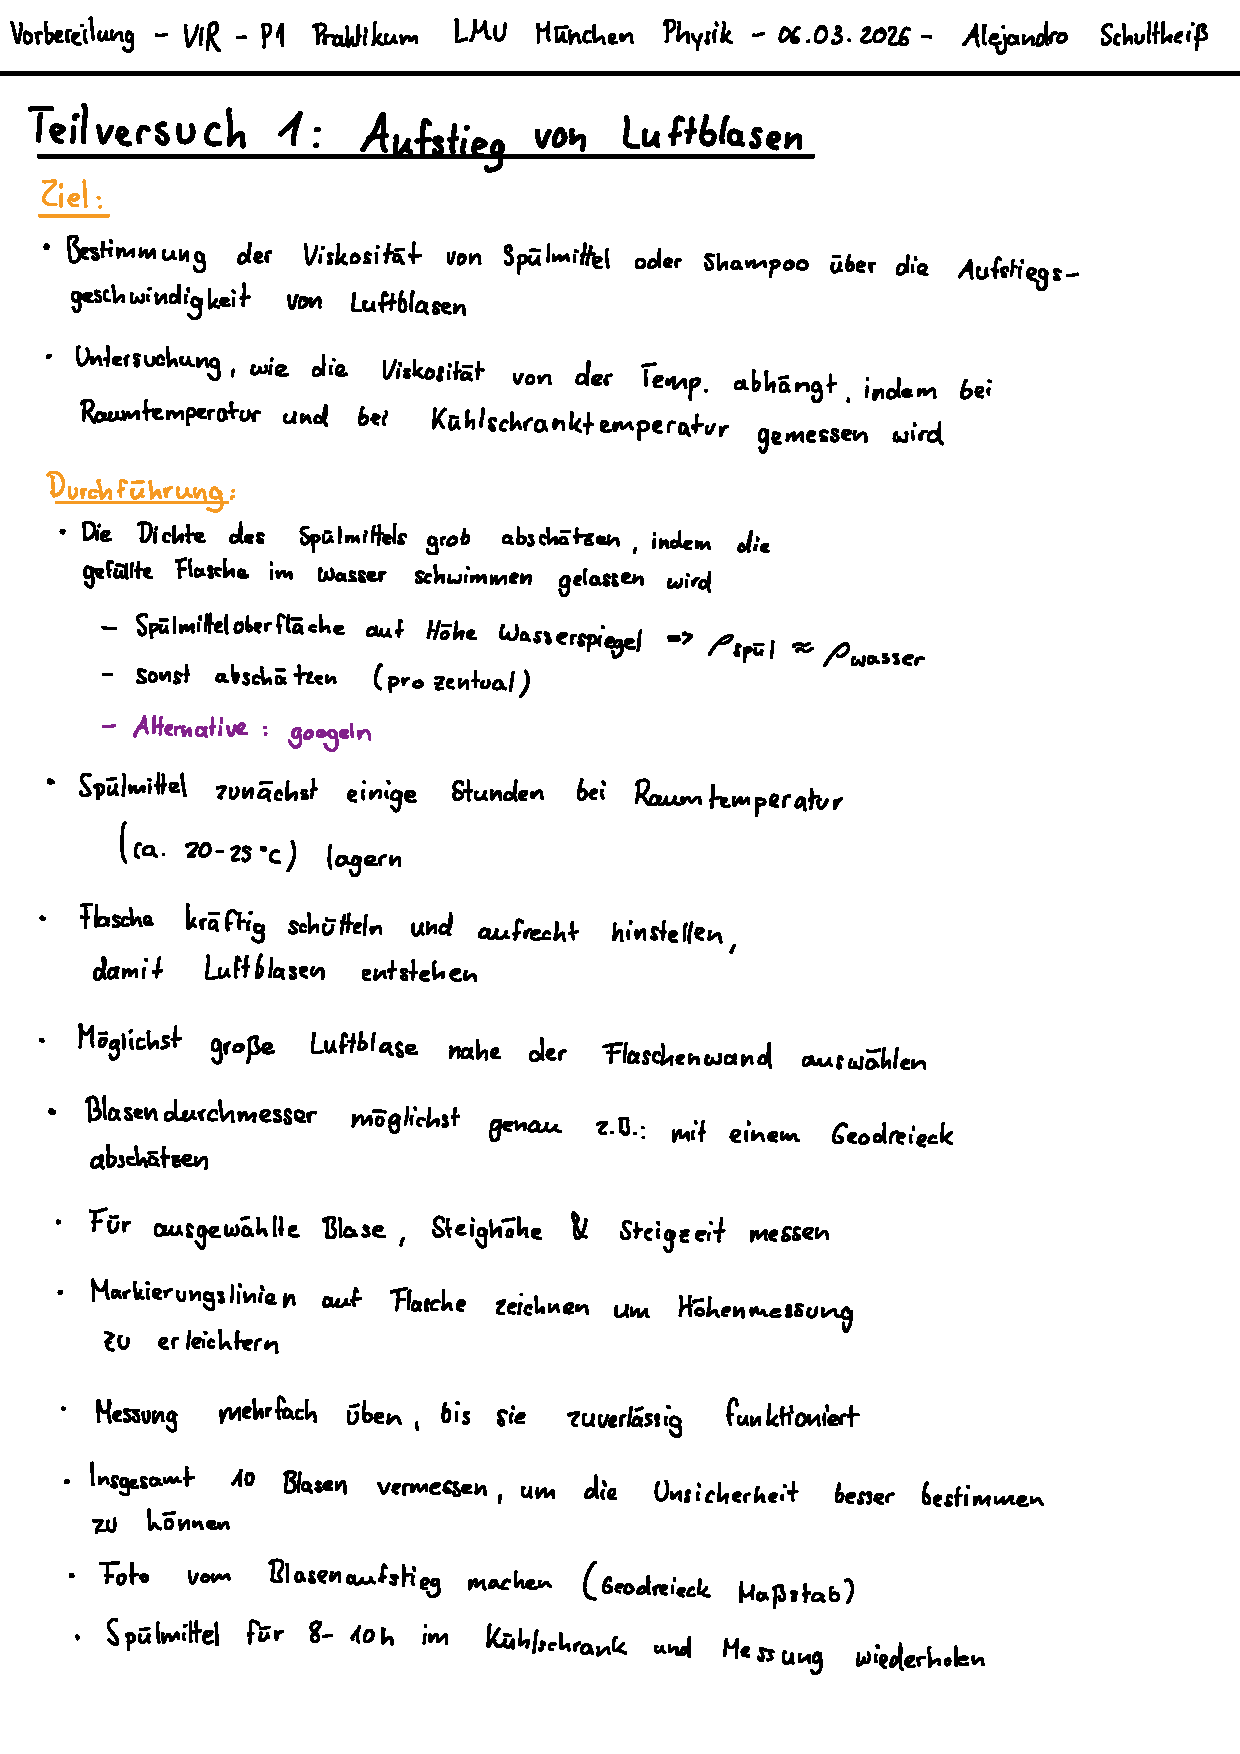
\includepdf[pages=-]{VIR_Vorbereitung_AS.pdf}

\newpage
\chapter{Durchführung Protokoll}
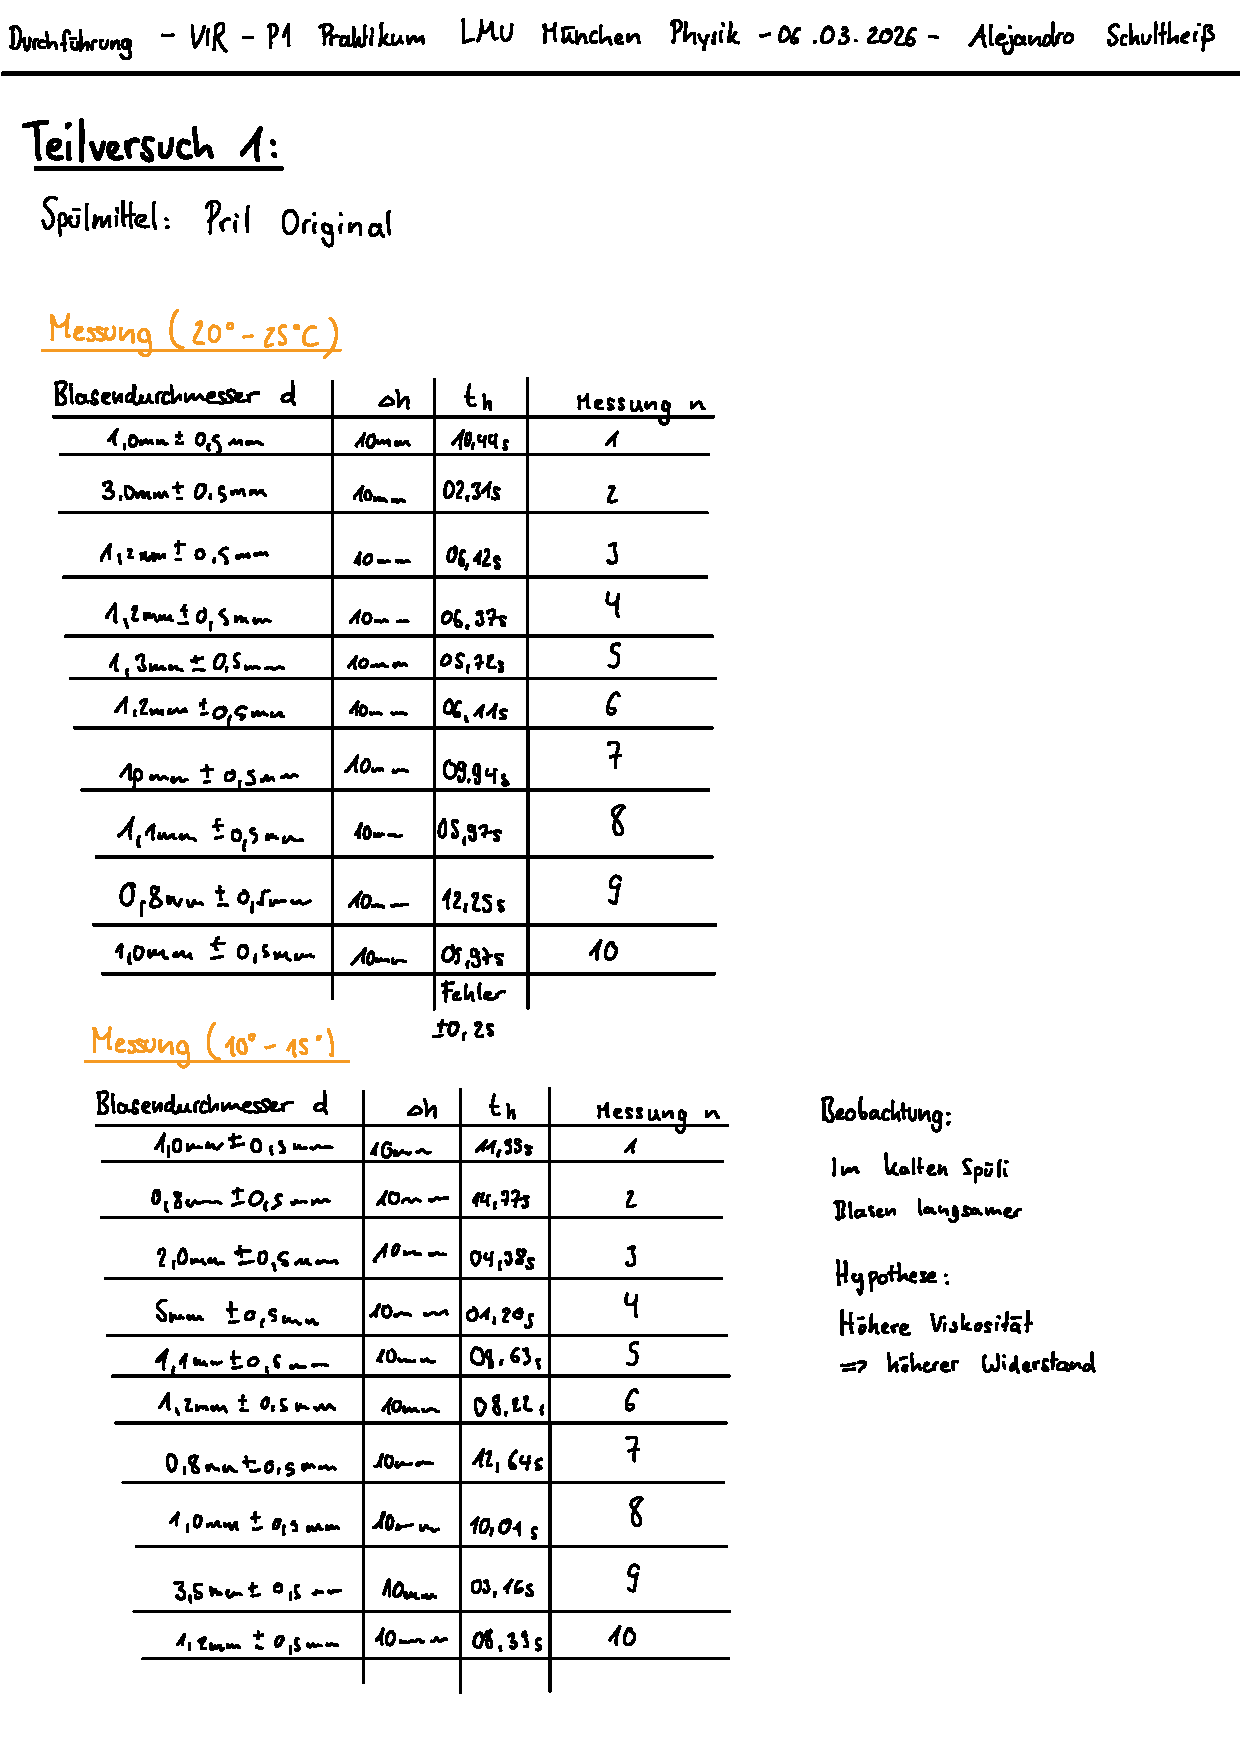
\includepdf[pages=-]{VIR_Durchfuehrung_AS.pdf}


\newpage
\chapter{Auswertung}
\section{Teilversuch I}

\begin{figure}[H]
    \centering
    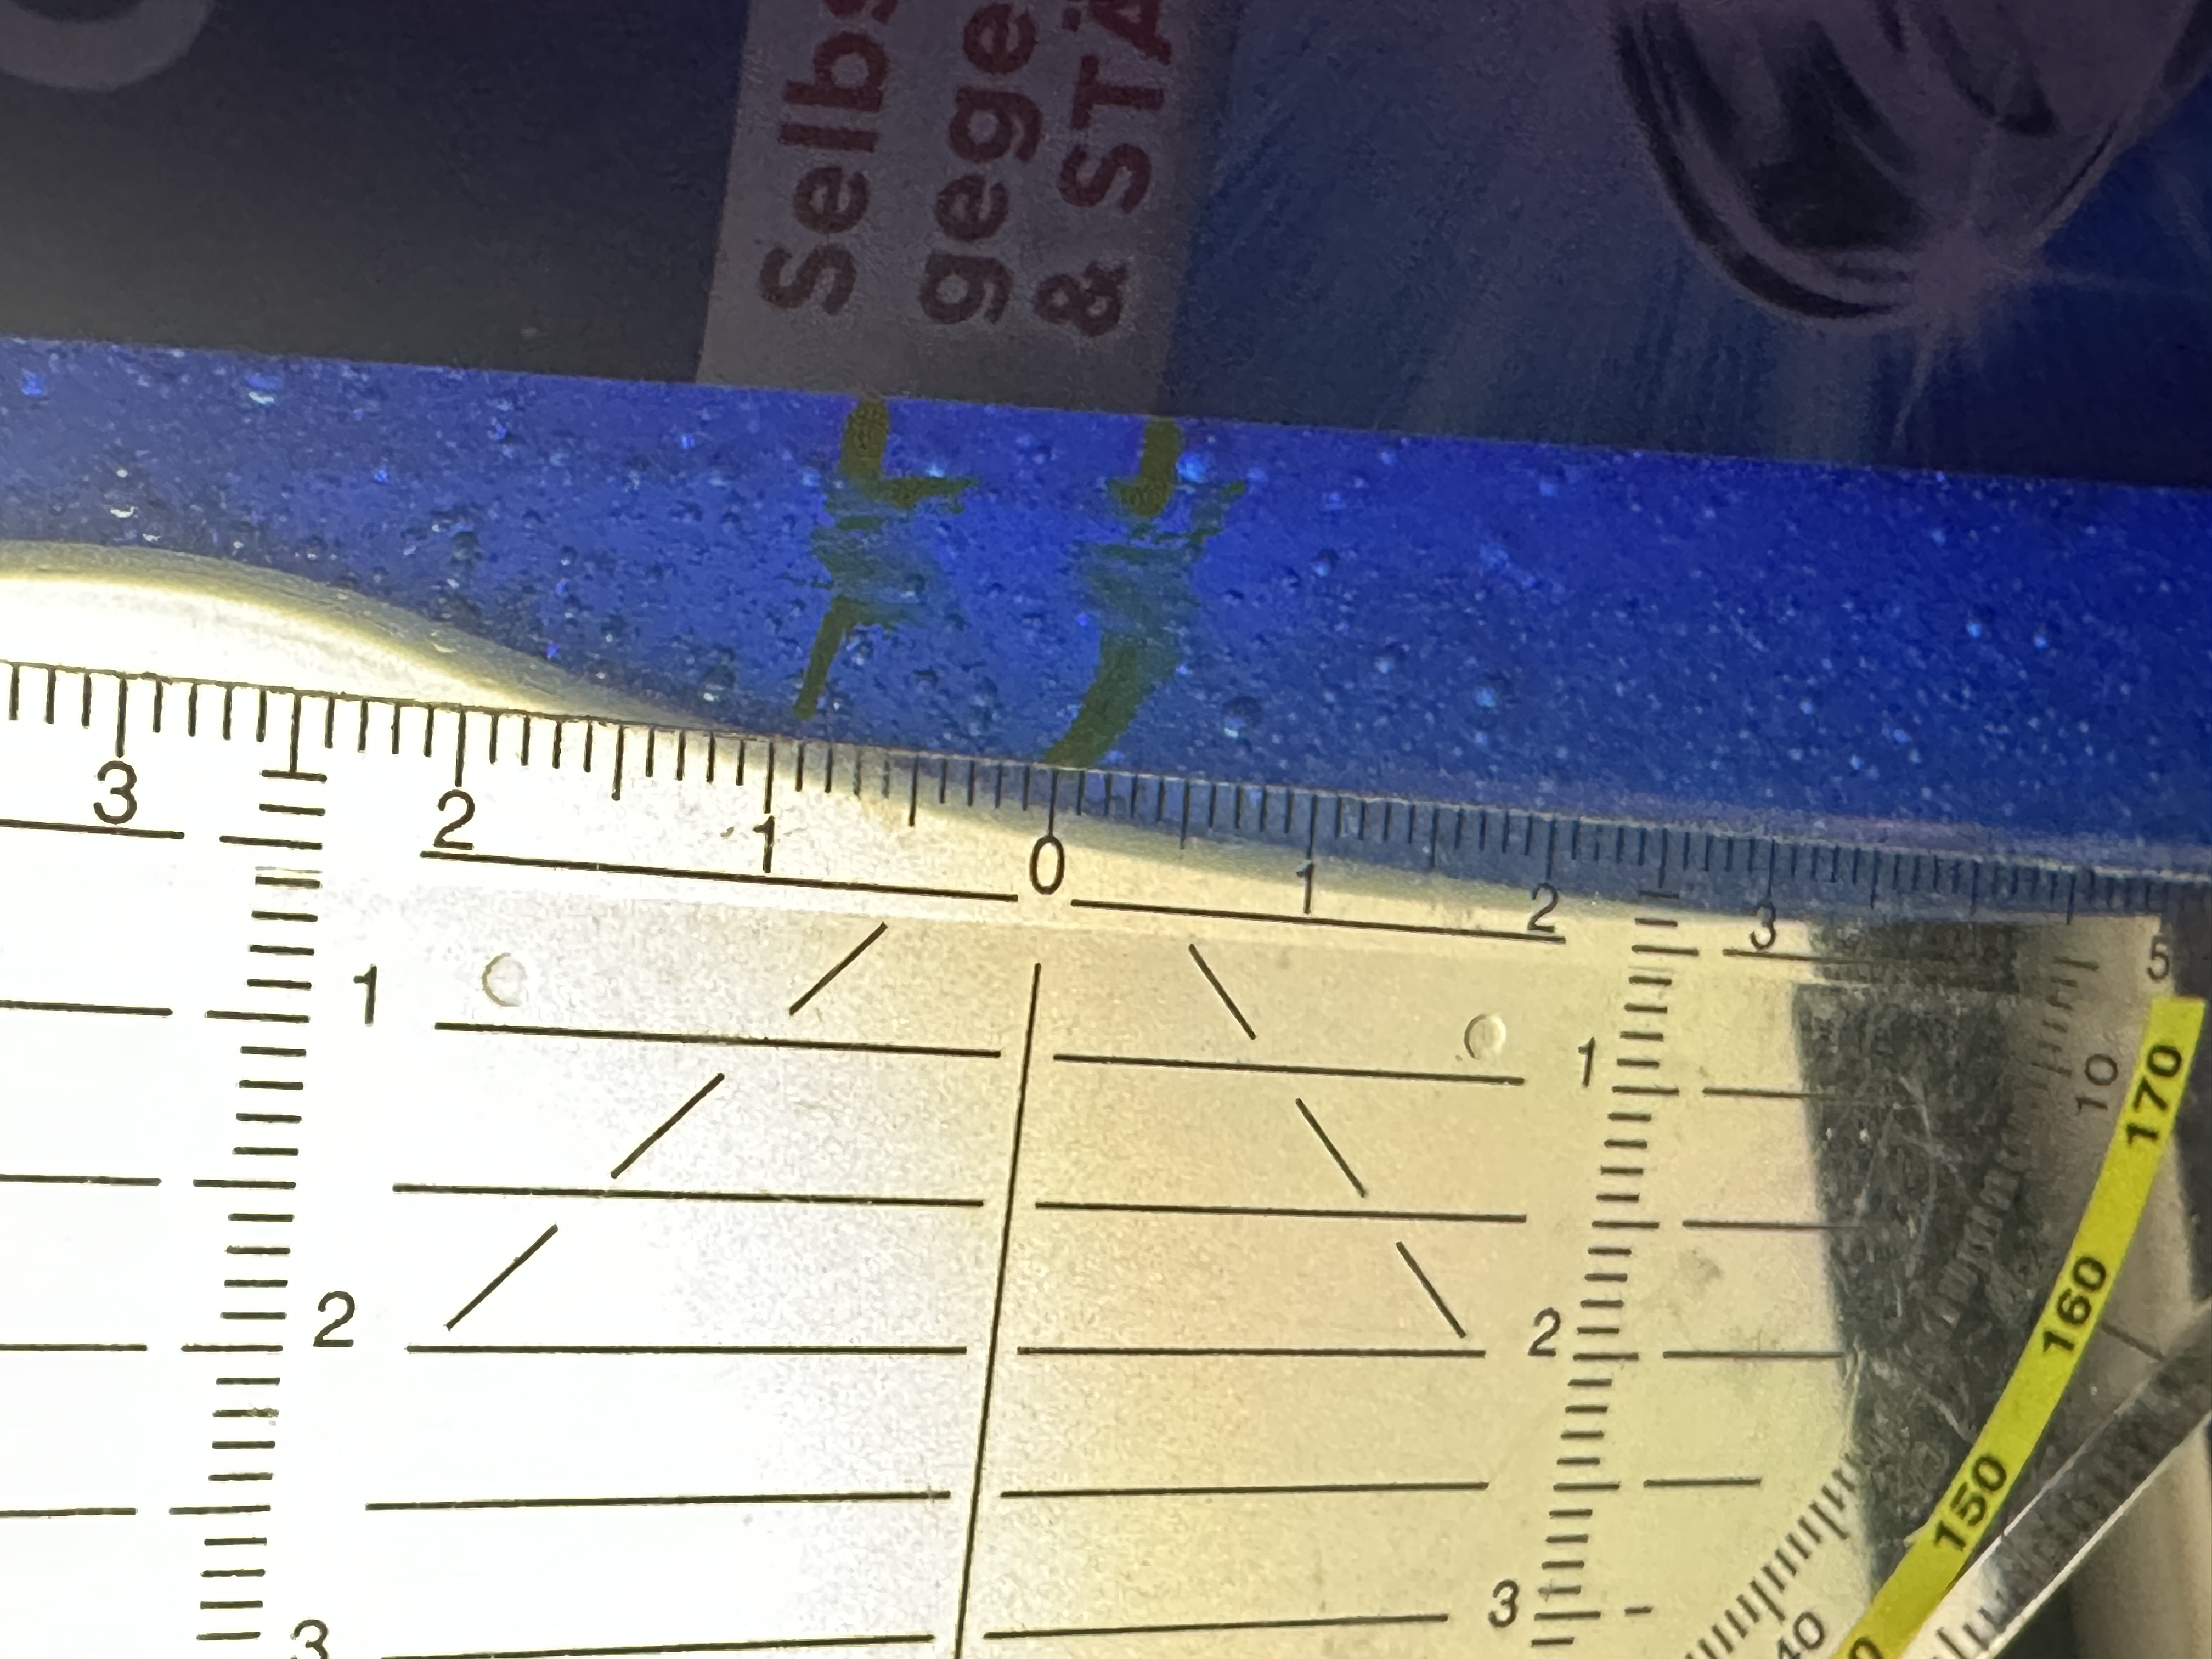
\includegraphics[width=0.8\textwidth]{IMG-0750.JPG}
    \caption{Viskosität in Abhängigkeit vom Blasendurchmesser für TV1.}
\end{figure}

Für den ersten Teilversuch wurde die Viskosität des Spülmittels aus der Aufstiegsgeschwindigkeit
von Luftblasen bestimmt. Die gemessene Steighöhe betrug in allen Messungen
\begin{equation}
    s = (10 \pm 1)\,\mathrm{mm} = (0{,}010 \pm 0{,}001)\,\mathrm{m}.
\end{equation}
Die Unsicherheiten der weiteren Messgrößen wurden zu
\begin{equation}
    \Delta d = 0{,}5\,\mathrm{mm},
    \qquad
    \Delta t = 0{,}2\,\mathrm{s}
\end{equation}
abgeschätzt. 
Für die Dichte des verwendeten Pril-Spülmittels wurde der Wert
\begin{equation}
    \rho = (1025 \pm 5)\,\mathrm{kg\,m^{-3}}
\end{equation}
verwendet.

\subsection{Verwendete Gleichungen}

Die Aufstiegsgeschwindigkeit der Blase ergibt sich aus
\begin{equation}
    v = \frac{s}{t}.
\end{equation}
Da in den Messwerten der Blasendurchmesser $d$ bestimmt wurde, gilt für den Radius
\begin{equation}
    r = \frac{d}{2}.
\end{equation}
Mit dem Stokesschen Gesetz folgt für die dynamische Viskosität
\begin{equation}
    \eta = \frac{2 g \rho}{9 v} r^2.
\end{equation}
Setzt man $v=s/t$ und $r=d/2$ ein, erhält man
\begin{equation}
    \eta = \frac{g \rho}{18}\,\frac{d^2 t}{s}.
\end{equation}

\subsection{Beispielrechnung}

Exemplarisch wird die erste Messung bei Raumtemperatur ausgewertet:
\begin{equation}
    d_1 = 1{,}0\,\mathrm{mm} = 1{,}0 \cdot 10^{-3}\,\mathrm{m},
    \qquad
    t_1 = 10{,}44\,\mathrm{s}.
\end{equation}
Damit folgt für den Radius
\begin{equation}
    r_1 = \frac{d_1}{2} = 0{,}5 \cdot 10^{-3}\,\mathrm{m}
\end{equation}
und für die Aufstiegsgeschwindigkeit
\begin{equation}
    v_1 = \frac{s}{t_1}
        = \frac{0{,}010\,\mathrm{m}}{10{,}44\,\mathrm{s}}
        \approx 9{,}58 \cdot 10^{-4}\,\mathrm{m\,s^{-1}}.
\end{equation}
Für die Viskosität ergibt sich damit
\begin{equation}
    \eta_1
    = \frac{2 \cdot 9{,}81\,\mathrm{m\,s^{-2}} \cdot 1025\,\mathrm{kg\,m^{-3}}}{9 \cdot 9{,}58 \cdot 10^{-4}\,\mathrm{m\,s^{-1}}}
      \left(0{,}5 \cdot 10^{-3}\,\mathrm{m}\right)^2
    \approx 0{,}583\,\mathrm{Pa\,s}.
\end{equation}

\subsection{Fehlerfortpflanzung}

Da
\begin{equation}
    \eta \propto \rho \, d^2 \, t \, s^{-1},
\end{equation}
ergibt sich für die relative Unsicherheit:
\begin{equation}
    \left(\frac{\Delta \eta}{\eta}\right)^2
    =
    \left(\frac{\Delta \rho}{\rho}\right)^2
    +
    \left(2\frac{\Delta d}{d}\right)^2
    +
    \left(\frac{\Delta t}{t}\right)^2
    +
    \left(\frac{\Delta s}{s}\right)^2.
\end{equation}
Die Unsicherheit der Viskosität berechnet sich damit zu
\begin{equation}
    \Delta \eta
    =
    \eta \,
    \sqrt{
    \left(\frac{\Delta \rho}{\rho}\right)^2
    +
    \left(2\frac{\Delta d}{d}\right)^2
    +
    \left(\frac{\Delta t}{t}\right)^2
    +
    \left(\frac{\Delta s}{s}\right)^2 }.
\end{equation}

\noindent
Es ist zu erwarten, dass die Unsicherheiten relativ groß werden, da die Steighöhe mit
nur $10\,\mathrm{mm}$ von mir sehr klein gewählt wurde. Dadurch wirkt sich die Unsicherheit
$\Delta s = 1\,\mathrm{mm}$ bereits mit einem relativen Fehler von $10\,\%$ aus.
Noch stärker fällt die Durchmesserunsicherheit ins Gewicht, da $\eta \sim d^2$ gilt.
Insbesondere bei kleinen Blasen führt $\Delta d = 0{,}5\,\mathrm{mm}$ zu sehr großen
relativen Fehlern.

\subsection{Messwerte und berechnete Viskositäten}

\subsubsection{Raumtemperatur}

\begin{table}[H]
\centering
\caption{Auswertung der Messwerte bei Raumtemperatur}
\begin{tabular}{c c c c c}
\toprule
Nr. & $d$ / mm & $t$ / s & $\eta$ / Pa\,s & $\Delta \eta$ / Pa\,s \\
\midrule
1  & 1{,}0 & 10{,}44 & 0{,}583 & 0{,}586 \\
2  & 3{,}0 & 2{,}31  & 1{,}161 & 0{,}417 \\
3  & 1{,}2 & 2{,}31  & 0{,}186 & 0{,}157 \\
4  & 1{,}2 & 6{,}37  & 0{,}512 & 0{,}430 \\
5  & 1{,}3 & 5{,}72  & 0{,}540 & 0{,}419 \\
6  & 1{,}2 & 6{,}11  & 0{,}492 & 0{,}413 \\
7  & 1{,}0 & 9{,}94  & 0{,}555 & 0{,}558 \\
8  & 1{,}1 & 5{,}97  & 0{,}404 & 0{,}369 \\
9  & 0{,}8 & 12{,}25 & 0{,}438 & 0{,}549 \\
10 & 1{,}0 & 5{,}97  & 0{,}333 & 0{,}335 \\
\bottomrule
\end{tabular}
\end{table}

Aus den zehn Einzelwerten ergibt sich der arithmetische Mittelwert
\begin{equation}
    \bar{\eta}_{\mathrm{RT}} = 0{,}520\,\mathrm{Pa\,s}.
\end{equation}
Die Standardabweichung der Einzelwerte beträgt
\begin{equation}
    \sigma_{\mathrm{RT}} = 0{,}255\,\mathrm{Pa\,s},
\end{equation}
und daraus folgt für den Fehler des Mittelwertes
\begin{equation}
    \Delta \bar{\eta}_{\mathrm{RT}}
    = \frac{\sigma_{\mathrm{RT}}}{\sqrt{10}}
    \approx 0{,}081\,\mathrm{Pa\,s}.
\end{equation}
Damit ergibt sich insgesamt
\begin{equation}
    \eta_{\mathrm{RT}} = (0{,}52 \pm 0{,}08)\,\mathrm{Pa\,s}.
\end{equation}

\subsubsection{Niedrige Temperatur}

\begin{table}[H]
\centering
\caption{Auswertung der Messwerte bei niedriger Temperatur}
\begin{tabular}{c c c c c}
\toprule
Nr. & $d$ / mm & $t$ / s & $\eta$ / Pa\,s & $\Delta \eta$ / Pa\,s \\
\midrule
1  & 1{,}0 & 11{,}35 & 0{,}634 & 0{,}637 \\
2  & 0{,}8 & 14{,}77 & 0{,}528 & 0{,}662 \\
3  & 2{,}0 & 4{,}38  & 0{,}979 & 0{,}501 \\
4  & 5{,}0 & 1{,}20  & 1{,}676 & 0{,}467 \\
5  & 1{,}1 & 8{,}63  & 0{,}583 & 0{,}534 \\
6  & 1{,}2 & 8{,}22  & 0{,}661 & 0{,}555 \\
7  & 0{,}8 & 12{,}64 & 0{,}452 & 0{,}567 \\
8  & 1{,}0 & 10{,}01 & 0{,}559 & 0{,}562 \\
9  & 3{,}5 & 3{,}16  & 2{,}162 & 0{,}669 \\
10 & 1{,}2 & 8{,}39  & 0{,}675 & 0{,}567 \\
\bottomrule
\end{tabular}
\end{table}

Für die Messreihe bei niedriger Temperatur ergibt sich der Mittelwert
\begin{equation}
    \bar{\eta}_{\mathrm{kalt}} = 0{,}891\,\mathrm{Pa\,s}.
\end{equation}
Die Standardabweichung der Einzelwerte beträgt
\begin{equation}
    \sigma_{\mathrm{kalt}} = 0{,}571\,\mathrm{Pa\,s},
\end{equation}
und damit folgt für den Fehler des Mittelwertes
\begin{equation}
    \Delta \bar{\eta}_{\mathrm{kalt}}
    = \frac{\sigma_{\mathrm{kalt}}}{\sqrt{10}}
    \approx 0{,}181\,\mathrm{Pa\,s}.
\end{equation}
Somit erhält man
\begin{equation}
    \eta_{\mathrm{kalt}} = (0{,}89 \pm 0{,}18)\,\mathrm{Pa\,s}.
\end{equation}

\subsection{Vergleich der Ergebnisse}

Die Viskosität des kalten Spülmittels ist deutlich größer als die bei Raumtemperatur:
\begin{equation}
    \eta_{\mathrm{kalt}} > \eta_{\mathrm{RT}}.
\end{equation}
Dies entspricht der Erwartung, da Flüssigkeiten bei sinkender Temperatur im Allgemeinen
zähflüssiger werden. Quantitativ ergibt sich ungefähr
\begin{equation}
    \frac{\eta_{\mathrm{kalt}}}{\eta_{\mathrm{RT}}}
    \approx 1{,}71.
\end{equation}
Das kalte Spülmittel besitzt also in dieser Messung eine etwa $1{,}7$-fach größere
Viskosität als das Spülmittel bei Raumtemperatur.

\subsection{Diskussion der Unsicherheiten}

Die berechneten Einzelwerte streuen relativ stark. Dies ist vor allem auf zwei Punkte
zurückzuführen:

\begin{enumerate}
    \item Die Steighöhe von nur $10\,\mathrm{mm}$ ist sehr klein. Dadurch führt bereits eine
    Unsicherheit von $1\,\mathrm{mm}$ zu einem relativen Fehler von $10\,\%$ in der
    Geschwindigkeit und damit auch in der Viskosität.

    \item Die Blasendurchmesser wurden nur grob abgeschätzt. Da die Viskosität quadratisch
    vom Durchmesser abhängt, wirkt sich dieser Fehler besonders stark aus. Für kleine
    Blasen wird der relative Fehler durch den Term $2\Delta d/d$ sehr groß und kann
    Werte von deutlich über $50\,\%$ erreichen.
\end{enumerate}

\noindent
Zusätzlich ist zu beachten, dass Luftblasen keine idealen starren Kugeln sind. Formabweichungen,
Wandnähe in der Flasche und mögliche Änderungen der Geschwindigkeit während des Aufstiegs
führen zu weiteren systematischen Abweichungen. Daher sind die ermittelten Werte eher als
Größenordnung der Viskosität zu verstehen.

\noindent
Trotz der großen Unsicherheiten zeigt die Messung jedoch klar den erwarteten Trend:
Bei niedriger Temperatur ist die Viskosität des Spülmittels größer als bei Raumtemperatur.


\begin{figure}[H]
    \centering
    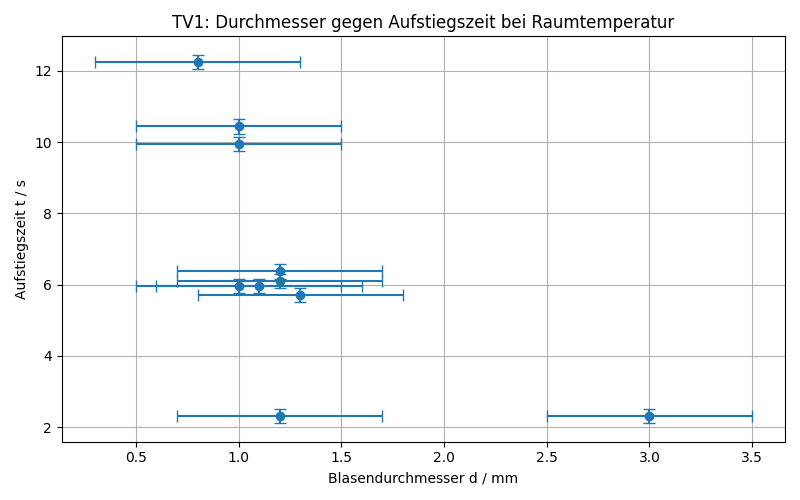
\includegraphics[width=0.8\textwidth]{Figure_1.png}
    \caption{Plot 1 TV1}
\end{figure}

\begin{figure}[H]
    \centering
    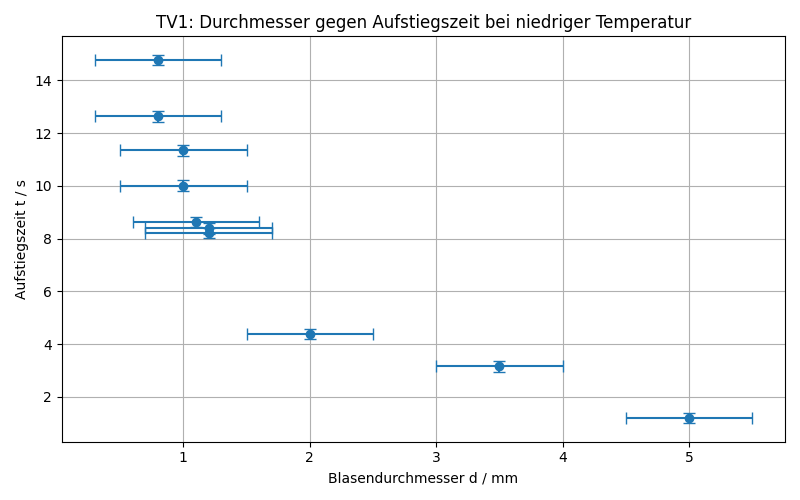
\includegraphics[width=0.8\textwidth]{Figure_2.png}
    \caption{Plot 2 TV1}
\end{figure}






\newpage
\section{Teilversuch II}

\begin{figure}[H]
    \centering
    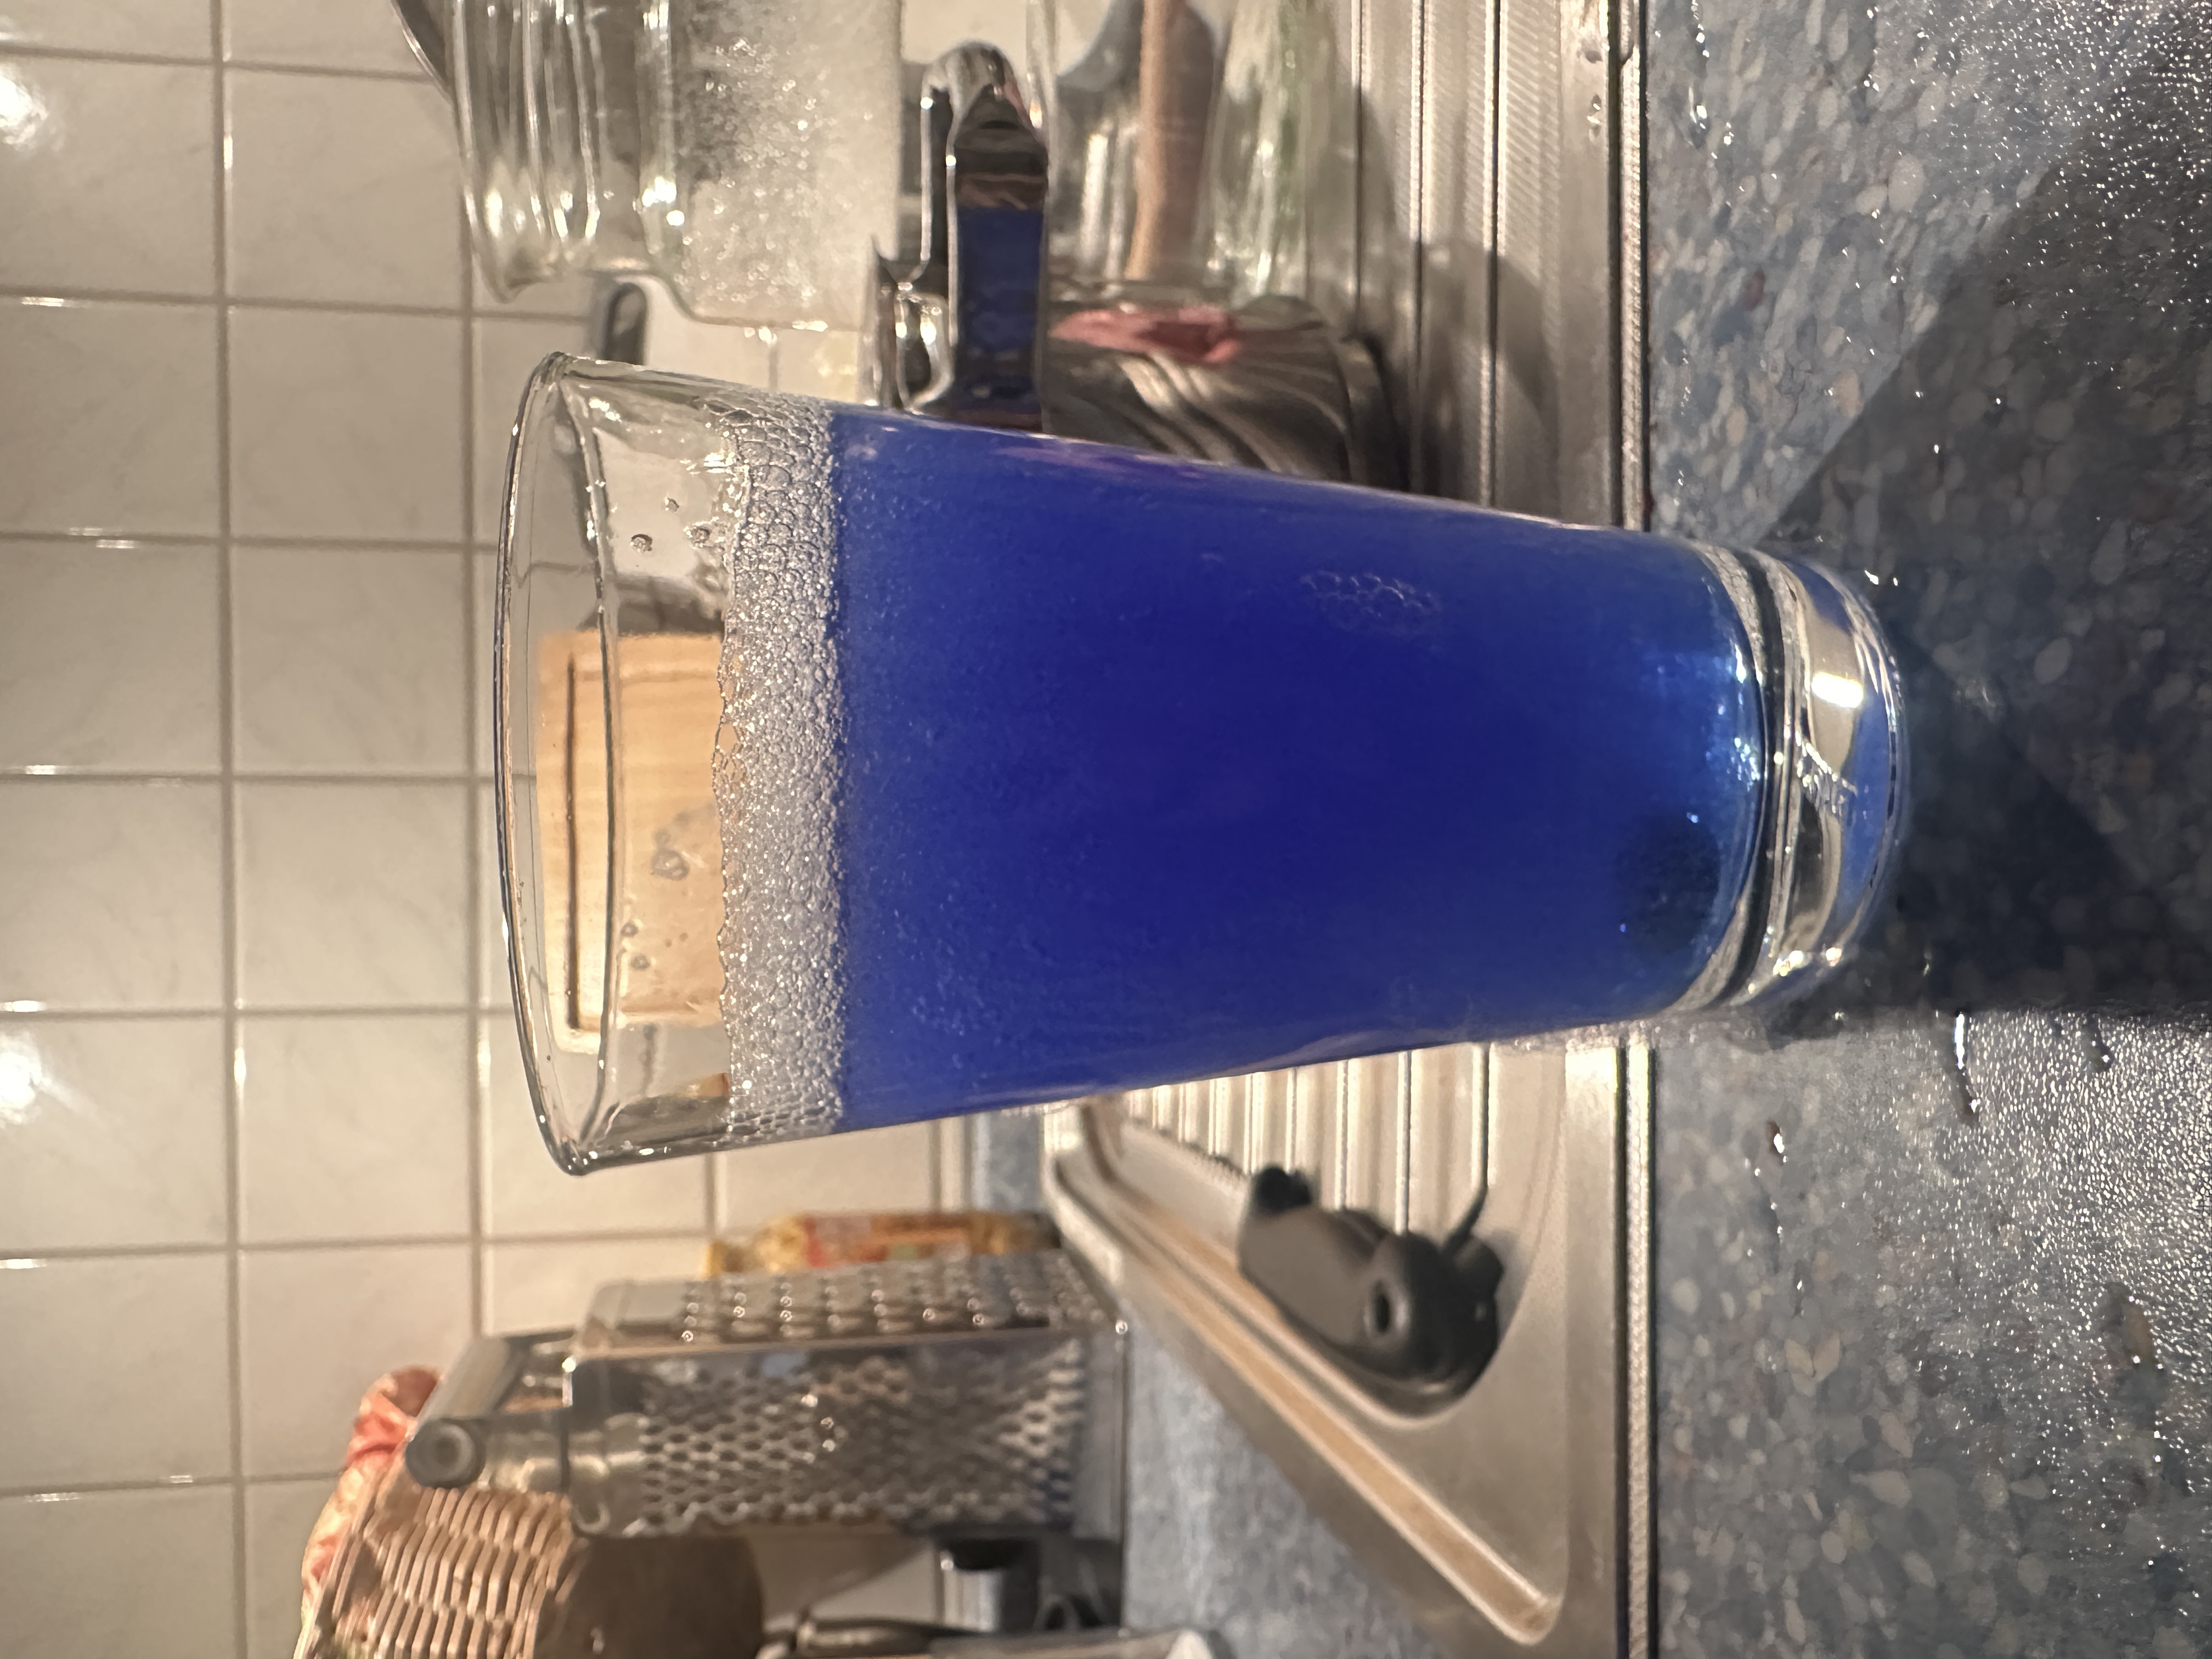
\includegraphics[width=0.8\textwidth]{IMG-0756.JPG}
    \caption{Viskosimeter}
\end{figure}
\begin{figure}[H]
    \centering
    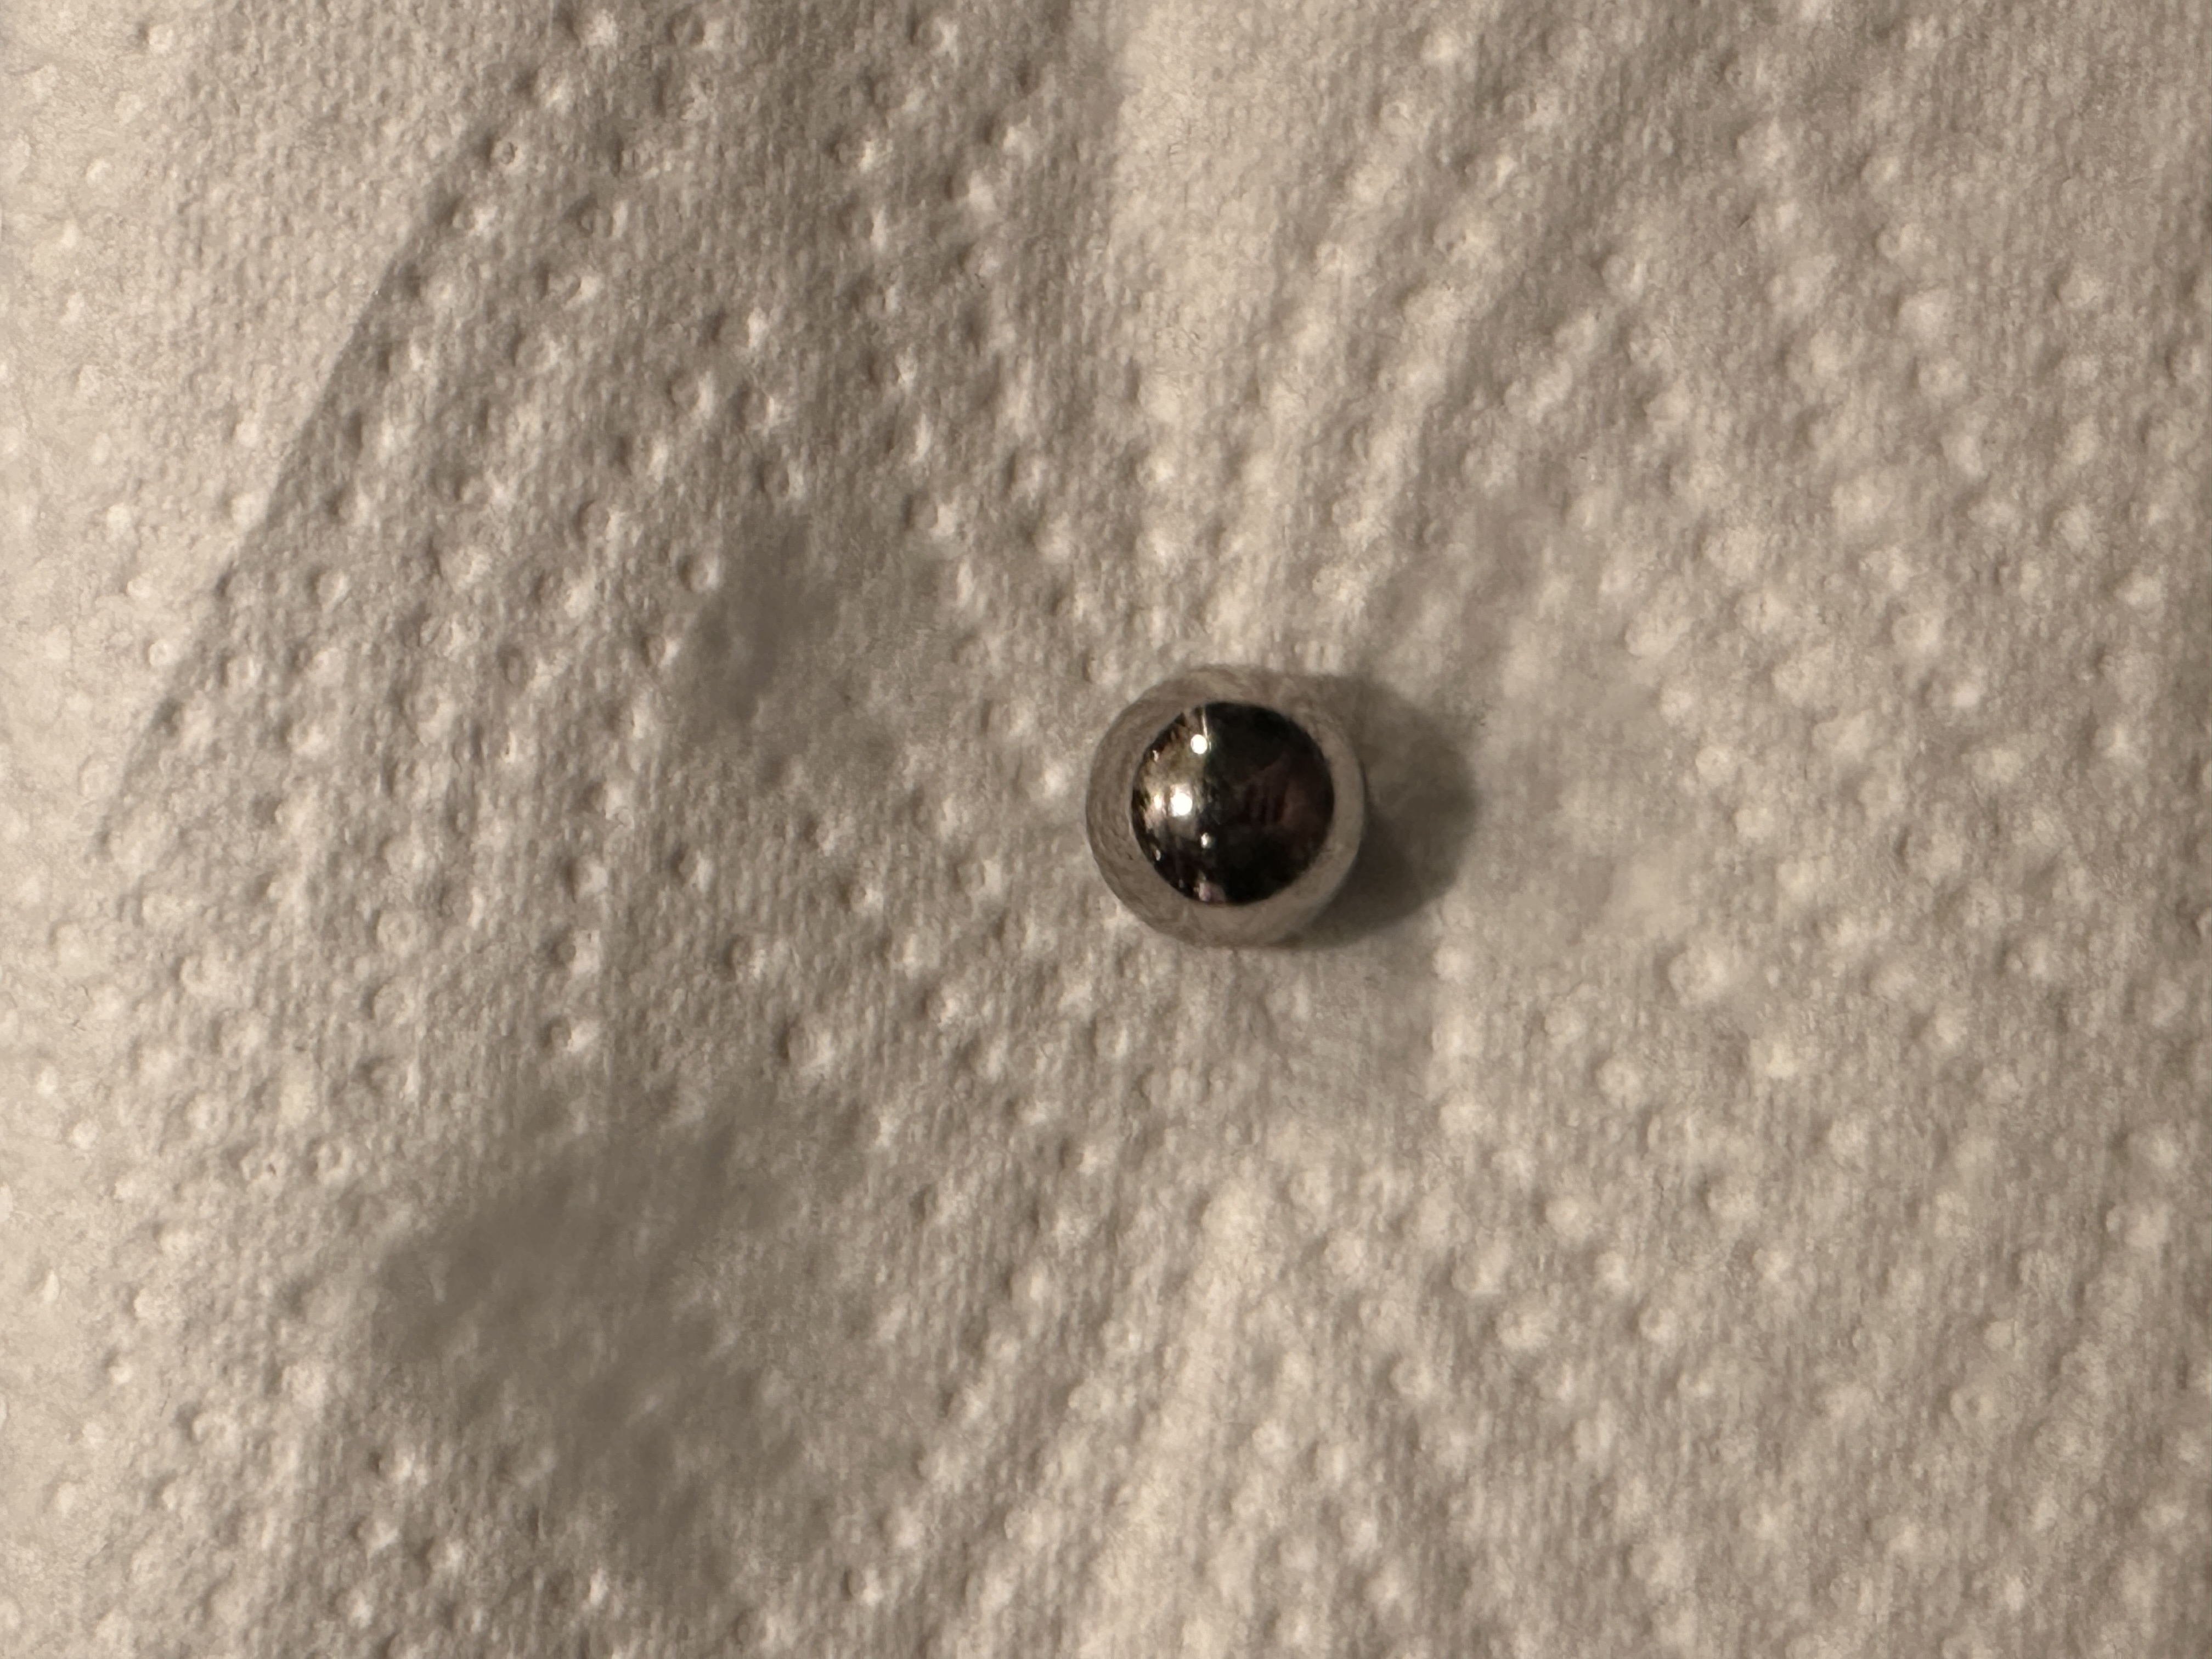
\includegraphics[width=0.8\textwidth]{IMG-0757.JPG}
    \caption{Stahlkugel}
\end{figure}




Für den zweiten Teilversuch wurde die Viskosität des Spülmittels mithilfe eines
einfachen Kugelfallviskosimeters bestimmt. Die Auswertung basiert auf einer
angenommenen Messreihe mit fünf Fallzeiten.

\noindent
Die verwendeten Größen sind:
\begin{equation}
    d = (1{,}20 \pm 0{,}05)\,\mathrm{cm} = (0{,}0120 \pm 0{,}0005)\,\mathrm{m},
\end{equation}
\begin{equation}
    r = \frac{d}{2} = (0{,}0060 \pm 0{,}00025)\,\mathrm{m},
\end{equation}
\begin{equation}
    m = (7{,}1 \pm 0{,}6)\,\mathrm{g} = (0{,}0071 \pm 0{,}0006)\,\mathrm{kg},
\end{equation}
\begin{equation}
    s = (6{,}0 \pm 0{,}2)\,\mathrm{cm} = (0{,}060 \pm 0{,}002)\,\mathrm{m}.
\end{equation}

\noindent
Für die Dichte des Spülmittels wurde wie in TV1 angesetzt:
\begin{equation}
    \rho_{\mathrm{Fl}} = (1025 \pm 5)\,\mathrm{kg\,m^{-3}}.
\end{equation}

\subsection{Dichte der Kugel}

Das Kugelvolumen beträgt
\begin{equation}
    V = \frac{4}{3}\pi r^3.
\end{equation}
Mit $r = 0{,}0060\,\mathrm{m}$ ergibt sich
\begin{equation}
    V = \frac{4}{3}\pi (0{,}0060\,\mathrm{m})^3
      \approx 9{,}05 \cdot 10^{-7}\,\mathrm{m^3}.
\end{equation}
Damit folgt für die Dichte der Kugel
\begin{equation}
    \rho_{\mathrm{K}} = \frac{m}{V}
    \approx \frac{0{,}0071\,\mathrm{kg}}{9{,}05 \cdot 10^{-7}\,\mathrm{m^3}}
    \approx 7{,}85 \cdot 10^3\,\mathrm{kg\,m^{-3}}.
\end{equation}
Dies ist plausibel für eine Stahlkugel. Im Folgenden wird daher verwendet:
\begin{equation}
    \rho_{\mathrm{K}} = (7850 \pm 700)\,\mathrm{kg\,m^{-3}}.
\end{equation}

\subsection{Verwendete Gleichungen}

Für die Fallgeschwindigkeit gilt
\begin{equation}
    v = \frac{s}{t}.
\end{equation}
\noindent
Mit dem Stokesschen Gesetz ergibt sich für die Viskosität:
\begin{equation}
    \eta = \frac{2}{9} \frac{r^2 g (\rho_{\mathrm{K}} - \rho_{\mathrm{Fl}})}{v}.
\end{equation}
\noindent
Setzt man $v = s/t$ ein, folgt
\begin{equation}
    \eta = \frac{2}{9} \frac{r^2 g (\rho_{\mathrm{K}} - \rho_{\mathrm{Fl}})\, t}{s}.
\end{equation}

\subsection{Messreihe}

Die verwendeten Fallzeiten lauten:
\begin{align}
    t_1 &= (1{,}42 \pm 0{,}10)\,\mathrm{s}, \\
    t_2 &= (1{,}36 \pm 0{,}10)\,\mathrm{s}, \\
    t_3 &= (1{,}39 \pm 0{,}10)\,\mathrm{s}, \\
    t_4 &= (1{,}47 \pm 0{,}10)\,\mathrm{s}, \\
    t_5 &= (1{,}33 \pm 0{,}10)\,\mathrm{s}.
\end{align}

\subsection{Beispielrechnung}

Exemplarisch wird die erste Messung ausgewertet:
\begin{equation}
    t_1 = 1{,}42\,\mathrm{s}.
\end{equation}
Daraus folgt für die Geschwindigkeit:
\begin{equation}
    v_1 = \frac{0{,}060\,\mathrm{m}}{1{,}42\,\mathrm{s}}
        \approx 4{,}23 \cdot 10^{-2}\,\mathrm{m\,s^{-1}}.
\end{equation}
\noindent
Die Viskosität ergibt sich zu
\begin{equation}
    \eta_1
    = \frac{2}{9}
      \frac{(0{,}0060\,\mathrm{m})^2 \cdot 9{,}81\,\mathrm{m\,s^{-2}}
      \cdot (7850 - 1025)\,\mathrm{kg\,m^{-3}}}
      {4{,}23 \cdot 10^{-2}\,\mathrm{m\,s^{-1}}}
    \approx 12{,}68\,\mathrm{Pa\,s}.
\end{equation}

\subsection{Fehlerfortpflanzung}

Da
\begin{equation}
    \eta \propto r^2 (\rho_{\mathrm{K}} - \rho_{\mathrm{Fl}})\, t\, s^{-1},
\end{equation}
ergibt sich näherungsweise für die relative Unsicherheit:
\begin{equation}
    \left(\frac{\Delta \eta}{\eta}\right)^2
    =
    \left(2\frac{\Delta r}{r}\right)^2
    +
    \left(\frac{\Delta(\rho_{\mathrm{K}}-\rho_{\mathrm{Fl}})}{\rho_{\mathrm{K}}-\rho_{\mathrm{Fl}}}\right)^2
    +
    \left(\frac{\Delta t}{t}\right)^2
    +
    \left(\frac{\Delta s}{s}\right)^2.
\end{equation}
\noindent
Mit den verwendeten Unsicherheiten ergibt sich eine relative Unsicherheit in der
Größenordnung von etwa $15\,\%$. Für die Einzelwerte ist daher näherungsweise
\begin{equation}
    \Delta \eta \approx 0{,}15 \,\eta
\end{equation}
anzusetzen.

\subsection{Berechnete Werte}

\begin{table}[H]
\centering
\caption{Auswertung der Messreihe für TV2}
\begin{tabular}{c c c c}
\toprule
Nr. & $t$ / s & $v$ / m\,s$^{-1}$ & $\eta$ / Pa\,s \\
\midrule
1 & 1{,}42 & 0{,}0423 & 12{,}68 \\
2 & 1{,}36 & 0{,}0441 & 12{,}14 \\
3 & 1{,}39 & 0{,}0432 & 12{,}41 \\
4 & 1{,}47 & 0{,}0408 & 13{,}12 \\
5 & 1{,}33 & 0{,}0451 & 11{,}87 \\
\bottomrule
\end{tabular}
\end{table}

Aus den fünf Einzelwerten ergibt sich der Mittelwert
\begin{equation}
    \bar{\eta}_{\mathrm{TV2}} = 12{,}44\,\mathrm{Pa\,s}.
\end{equation}
\noindent
Die Standardabweichung der Einzelwerte beträgt
\begin{equation}
    \sigma = 0{,}48\,\mathrm{Pa\,s},
\end{equation}
und damit folgt für den Fehler des Mittelwertes
\begin{equation}
    \Delta \bar{\eta}_{\mathrm{TV2}}
    = \frac{\sigma}{\sqrt{5}}
    \approx 0{,}22\,\mathrm{Pa\,s}.
\end{equation}
\noindent
Berücksichtigt man zusätzlich die systematischen Unsicherheiten von Kugelradius,
Kugeldichte und Fallstrecke, so ist ein deutlich größerer Gesamtfehler anzusetzen.
Daher wird als Endergebnis sinnvoll angegeben:
\begin{equation}
    \eta_{\mathrm{TV2}} = (12{,}4 \pm 1{,}9)\,\mathrm{Pa\,s}.
\end{equation}

\subsection{Diskussion}

Der für TV2 erhaltene Wert liegt deutlich über den in TV1 bestimmten Werten. Dies kann
mehrere Ursachen haben. Zum einen ist das Kugelfallviskosimeter hier nur sehr einfach
aufgebaut, sodass Wandnähe, ungenaue Fallstrecke und eine möglicherweise noch nicht
vollständig erreichte Endgeschwindigkeit der Kugel das Ergebnis beeinflussen. Zum anderen
beruht die Auswertung auf einer grob abgeschätzten Kugelmasse sowie auf der Annahme, dass
es sich tatsächlich um eine Stahlkugel handelt.
\noindent
Trotzdem zeigt die Messreihe eine vergleichsweise geringe Streuung der Einzelwerte.
Die Präzision innerhalb der Reihe ist also recht gut, während die absolute Genauigkeit
wegen der systematischen Unsicherheiten begrenzt ist.
\noindent
Insgesamt liefert TV2 damit einen plausiblen Größenordnungswert für eine stark viskose
Flüssigkeit, ist jedoch deutlich unsicherer als ein kalibriertes Kugelfallviskosimeter.



\newpage
\chapter{Anhang}
\section{SCRIPTS}

\begin{lstlisting}[caption={Python-Skript zur Darstellung von TV1 mit Fehlerbalken}]
import numpy as np
import matplotlib.pyplot as plt

# Unsicherheit
d_err = 0.5
t_err = 0.2

# Normale Temp
d_rt = np.array([1.0, 3.0, 1.2, 1.2, 1.3, 1.2, 1.0, 1.1, 0.8, 1.0])
t_rt = np.array([10.44, 2.31, 2.31, 6.37, 5.72, 6.11, 9.94, 5.97, 12.25, 5.97])

# Kalt
d_kalt = np.array([1.0, 0.8, 2.0, 5.0, 1.1, 1.2, 0.8, 1.0, 3.5, 1.2])
t_kalt = np.array([11.35, 14.77, 4.38, 1.20, 8.63, 8.22, 12.64, 10.01, 3.16, 8.39])

# Fehlerarrays
d_rt_err = np.full_like(d_rt, d_err, dtype=float)
t_rt_err = np.full_like(t_rt, t_err, dtype=float)

d_kalt_err = np.full_like(d_kalt, d_err, dtype=float)
t_kalt_err = np.full_like(t_kalt, t_err, dtype=float)

# Plot 1
plt.figure(figsize=(8, 5))
plt.errorbar(
    d_rt, t_rt,
    xerr=d_rt_err, yerr=t_rt_err,
    fmt='o', capsize=4
)
plt.xlabel('Blasendurchmesser d / mm')
plt.ylabel('Aufstiegszeit t / s')
plt.title('TV1: Durchmesser gegen Aufstiegszeit bei Raumtemperatur')
plt.grid(True)
plt.tight_layout()
plt.savefig('TV1_Raumtemperatur_Durchmesser_Zeit.png', dpi=300)
plt.show()

# Plot 2: Kalt
plt.figure(figsize=(8, 5))
plt.errorbar(
    d_kalt, t_kalt,
    xerr=d_kalt_err, yerr=t_kalt_err,
    fmt='o', capsize=4
)
plt.xlabel('Blasendurchmesser d / mm')
plt.ylabel('Aufstiegszeit t / s')
plt.title('TV1: Durchmesser gegen Aufstiegszeit bei niedriger Temperatur')
plt.grid(True)
plt.tight_layout()
plt.savefig('TV1_Kalt_Durchmesser_Zeit.png', dpi=300)
plt.show()
\end{lstlisting}








\end{document}
